% !TeX program = xelatex
\documentclass[UTF8,12pt,a4paper]{ctexart}
\usepackage{amsmath,amssymb}
\usepackage{geometry}
\usepackage{tikz}
\geometry{margin=2cm}

% ===== 水印：贺昱超学习资料 =====
\usepackage{xcolor}
\usepackage{eso-pic}
\usepackage{graphicx}

\newcommand{\WMText}{贺昱超专属测试卷}
\newcommand{\WMScale}{2.28}
\newcommand{\WMAngle}{45}
\colorlet{WMColor}{black!8}

\AddToShipoutPictureBG{%
  \AtPageLowerLeft{%
    \put(\LenToUnit{0.66\paperwidth},\LenToUnit{0.70\paperheight}){%
      \rotatebox{\WMAngle}{\scalebox{\WMScale}{\textcolor{WMColor}{\WMText}}}%
    }%
    \put(\LenToUnit{0.33\paperwidth},\LenToUnit{0.50\paperheight}){%
      \rotatebox{\WMAngle}{\scalebox{\WMScale}{\textcolor{WMColor}{\WMText}}}%
    }%
    \put(\LenToUnit{0.66\paperwidth},\LenToUnit{0.30\paperheight}){%
      \rotatebox{\WMAngle}{\scalebox{\WMScale}{\textcolor{WMColor}{\WMText}}}%
    }%
  }%
}

% ===== 8题铺满一页布局 =====
\usepackage{enumitem}
\newcommand{\BottomWriteSpace}{0.5cm}

\newenvironment{OnePageEightFill}{
  \small
  \vspace*{0pt}
  \begin{enumerate}[leftmargin=*, itemsep=0pt, topsep=0pt, parsep=0pt, partopsep=0pt]
  \setlength{\parskip}{0pt}
}{
  \end{enumerate}
  \vspace*{\BottomWriteSpace}
  \normalsize
  \newpage
}

\newcommand{\Q}[1]{\item #1\par\vfill}
\newcommand{\Qlast}[1]{\item #1\par}

\begin{document}

% =========================================================
% 7.27
% =========================================================
\section*{7月27日作业（8道题当晚22:00前打卡）}
\begin{OnePageEightFill}

\Q{计算：$\displaystyle \frac{2024 + \dfrac{1}{2023}}{2023 + \dfrac{1}{2024}} - \frac{2022 + \dfrac{1}{2023}}{2023 + \dfrac{1}{2022}}$}

\Q{解方程组：$\begin{cases} 2x - y = 3 \\ \dfrac{x-1}{2} = \dfrac{y-3}{3} \end{cases}$}

\Q{
\begin{minipage}[c]{0.75\textwidth}
如图，为一个 3 行 3 列的表格，当空格内填上适当的数后，每行、每列以及每条对角线上的数字之和都是相等的，则 $k =$ \underline{\hspace{3em}}。
\end{minipage}
\hfill
\begin{minipage}[c]{0.2\textwidth}
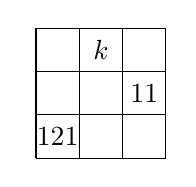
\begin{tikzpicture}[scale=0.55]
  \draw (0,0) grid (3,3);
  \node at (0.5, 0.5) {121};
  \node at (2.5, 1.5) {11};
  \node at (1.5, 2.5) {$k$};
\end{tikzpicture}
\end{minipage}
}

\Q{A、B 两地之间是山路，相距 240 千米，其中一部分是上坡路，其余是下坡路。某人骑电动车从 A 地到 B 地，再沿原路返回，去时用了 11 小时，返回时用了 9 小时。已知下坡路每小时行驶 30 千米，那么上坡路每小时行驶多少千米？}

\Q{
\begin{minipage}[c]{0.75\textwidth}
如图，$\triangle ABC$ 的面积是 36 平方厘米，$AD=DE=EC$，$F$ 是 $BC$ 中点，$FG=GC$，阴影部分的面积是\underline{\hspace{3em}}平方厘米。
\end{minipage}
\hfill
\begin{minipage}[c]{0.2\textwidth}
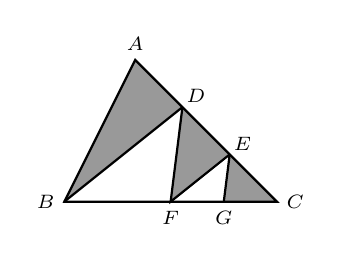
\begin{tikzpicture}[scale=0.45]
  \coordinate (B) at (0,0); \coordinate (C) at (6,0); \coordinate (A) at (2,4);
  \coordinate (D) at (3.333, 2.667); \coordinate (E) at (4.667, 1.333);
  \coordinate (F) at (3,0); \coordinate (G) at (4.5,0);
  \fill[gray!80] (A) -- (B) -- (D) -- cycle;
  \fill[gray!80] (D) -- (E) -- (F) -- cycle;
  \fill[gray!80] (E) -- (G) -- (C) -- cycle;
  \draw[thick] (A) -- (B) -- (C) -- cycle;
  \draw[thick] (B) -- (D); \draw[thick] (D) -- (F) -- (E); \draw[thick] (E) -- (G);
  \node[above] at (A) {\scriptsize $A$}; \node[left] at (B) {\scriptsize $B$}; \node[right] at (C) {\scriptsize $C$};
  \node[above right=-2pt] at (D) {\scriptsize $D$}; \node[above right=-2pt] at (E) {\scriptsize $E$};
  \node[below] at (F) {\scriptsize $F$}; \node[below] at (G) {\scriptsize $G$};
\end{tikzpicture}
\end{minipage}
}

\Q{桌上放有一张写有 61 的卡片，若从桌子的另一侧看去，却是 19。现在桌子上放着这样一道算术题：$89 + 16 + 69 + 6\Box + \Box8$。甲、乙两位同学面对面坐在桌子两侧，而他们计算这道数学题的结果恰好相同，则两个方格中应填的数字和是\underline{\hspace{3em}}。}

\Q{一列火车出发 1 小时后因故停车 0.5 小时，然后以原速的 $\dfrac{3}{4}$ 前进，最终到达目的地晚 1.5 小时。若出发 1 小时后又前进 90 公里再因故停车 0.5 小时，然后同样以原速的 $\dfrac{3}{4}$ 前进，则到达目的地仅晚 1 小时。那么整个路程为多少公里？}

\Qlast{老师在黑板上写了若干个从 1 开始的连续自然数：$1, 2, 3, 4, \dots$，后来擦掉其中的一个，剩下的数的平均数是 $13\dfrac{9}{13}$，擦掉的自然数是\underline{\hspace{3em}}。}

\end{OnePageEightFill}

% =========================================================
% 7.28
% =========================================================
\section*{7月28日作业（8道题当晚22:00前打卡）}
\begin{OnePageEightFill}

\Q{计算：$\displaystyle \frac{100 + \dfrac{1}{99}}{99 + \dfrac{1}{100}} - \frac{98 + \dfrac{1}{99}}{99 + \dfrac{1}{98}}$}

\Q{解方程组：$\begin{cases} 3x - y = 5 \\ \dfrac{x+2}{4} = \dfrac{y-1}{2} \end{cases}$}

\Q{
\begin{minipage}[c]{0.75\textwidth}
如图，为一个 3 行 3 列的表格，当空格内填上适当的数后，每行、每列以及每条对角线上的数字之和都是相等的，则 $k =$ \underline{\hspace{3em}}。
\end{minipage}
\hfill
\begin{minipage}[c]{0.2\textwidth}
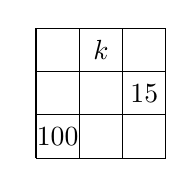
\begin{tikzpicture}[scale=0.55]
  \draw (0,0) grid (3,3);
  \node at (0.5, 0.5) {100};
  \node at (2.5, 1.5) {15};
  \node at (1.5, 2.5) {$k$};
\end{tikzpicture}
\end{minipage}
}

\Q{A、B 两地之间是山路，相距 180 千米，其中一部分是上坡路，其余是下坡路。某人骑电动车从 A 地到 B 地，再沿原路返回，去时用了 8 小时，返回时用了 7 小时。已知下坡路每小时行驶 30 千米，那么上坡路每小时行驶多少千米？}

\Q{
\begin{minipage}[c]{0.75\textwidth}
如图，$\triangle ABC$ 的面积是 48 平方厘米，$AD=DE=EC$，$F$ 是 $BC$ 中点，$FG=GC$，阴影部分的面积是\underline{\hspace{3em}}平方厘米。
\end{minipage}
\hfill
\begin{minipage}[c]{0.2\textwidth}
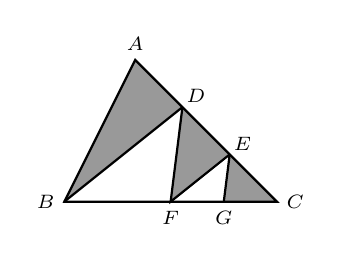
\begin{tikzpicture}[scale=0.45]
  \coordinate (B) at (0,0); \coordinate (C) at (6,0); \coordinate (A) at (2,4);
  \coordinate (D) at (3.333, 2.667); \coordinate (E) at (4.667, 1.333);
  \coordinate (F) at (3,0); \coordinate (G) at (4.5,0);
  \fill[gray!80] (A) -- (B) -- (D) -- cycle;
  \fill[gray!80] (D) -- (E) -- (F) -- cycle;
  \fill[gray!80] (E) -- (G) -- (C) -- cycle;
  \draw[thick] (A) -- (B) -- (C) -- cycle;
  \draw[thick] (B) -- (D); \draw[thick] (D) -- (F) -- (E); \draw[thick] (E) -- (G);
  \node[above] at (A) {\scriptsize $A$}; \node[left] at (B) {\scriptsize $B$}; \node[right] at (C) {\scriptsize $C$};
  \node[above right=-2pt] at (D) {\scriptsize $D$}; \node[above right=-2pt] at (E) {\scriptsize $E$};
  \node[below] at (F) {\scriptsize $F$}; \node[below] at (G) {\scriptsize $G$};
\end{tikzpicture}
\end{minipage}
}

\Q{桌上放有一张写有 61 的卡片，若从桌子的另一侧看去，却是 19。现在桌子上放着这样一道算术题：$89 + 81 + 69 + 6\Box + \Box8$。甲、乙两位同学面对面坐在桌子两侧，而他们计算这道数学题的结果恰好相同，则两个方格中应填的数字和是\underline{\hspace{3em}}。}

\Q{一列火车出发 2 小时后因故停车 0.5 小时，然后以原速的 $\dfrac{4}{5}$ 前进，最终到达目的地晚 1.5 小时。若出发 2 小时后又前进 120 公里再因故停车 0.5 小时，然后同样以原速的 $\dfrac{4}{5}$ 前进，则到达目的地仅晚 1 小时。那么整个路程为多少公里？}

\Qlast{老师在黑板上写了若干个从 1 开始的连续自然数：$1, 2, 3, 4, \dots$，后来擦掉其中的一个，剩下的数的平均数是 $16\dfrac{4}{15}$，擦掉的自然数是\underline{\hspace{3em}}。}

\end{OnePageEightFill}

% =========================================================
% 7.29
% =========================================================
\section*{7月29日作业（8道题当晚22:00前打卡）}
\begin{OnePageEightFill}

\Q{计算：$\displaystyle \frac{50 + \dfrac{1}{49}}{49 + \dfrac{1}{50}} - \frac{48 + \dfrac{1}{49}}{49 + \dfrac{1}{48}}$}

\Q{解方程组：$\begin{cases} 4x + 5y = 23 \\ \dfrac{x+1}{2} = \dfrac{y+2}{3} \end{cases}$}

\Q{
\begin{minipage}[c]{0.75\textwidth}
如图，为一个 3 行 3 列的表格，当空格内填上适当的数后，每行、每列以及每条对角线上的数字之和都是相等的，则 $k =$ \underline{\hspace{3em}}。
\end{minipage}
\hfill
\begin{minipage}[c]{0.2\textwidth}
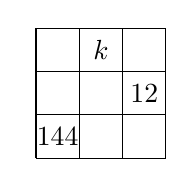
\begin{tikzpicture}[scale=0.55]
  \draw (0,0) grid (3,3);
  \node at (0.5, 0.5) {144};
  \node at (2.5, 1.5) {12};
  \node at (1.5, 2.5) {$k$};
\end{tikzpicture}
\end{minipage}
}

\Q{A、B 两地之间是山路，相距 300 千米，其中一部分是上坡路，其余是下坡路。某人骑电动车从 A 地到 B 地，再沿原路返回，去时用了 13 小时，返回时用了 12 小时。已知下坡路每小时行驶 30 千米，那么上坡路每小时行驶多少千米？}

\Q{
\begin{minipage}[c]{0.75\textwidth}
如图，$\triangle ABC$ 的面积是 60 平方厘米，$AD=DE=EC$，$F$ 是 $BC$ 中点，$FG=GC$，阴影部分的面积是\underline{\hspace{3em}}平方厘米。
\end{minipage}
\hfill
\begin{minipage}[c]{0.2\textwidth}
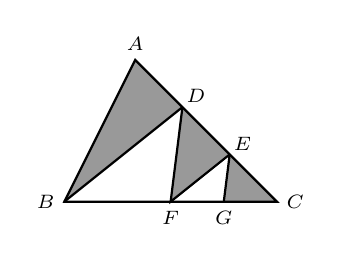
\begin{tikzpicture}[scale=0.45]
  \coordinate (B) at (0,0); \coordinate (C) at (6,0); \coordinate (A) at (2,4);
  \coordinate (D) at (3.333, 2.667); \coordinate (E) at (4.667, 1.333);
  \coordinate (F) at (3,0); \coordinate (G) at (4.5,0);
  \fill[gray!80] (A) -- (B) -- (D) -- cycle;
  \fill[gray!80] (D) -- (E) -- (F) -- cycle;
  \fill[gray!80] (E) -- (G) -- (C) -- cycle;
  \draw[thick] (A) -- (B) -- (C) -- cycle;
  \draw[thick] (B) -- (D); \draw[thick] (D) -- (F) -- (E); \draw[thick] (E) -- (G);
  \node[above] at (A) {\scriptsize $A$}; \node[left] at (B) {\scriptsize $B$}; \node[right] at (C) {\scriptsize $C$};
  \node[above right=-2pt] at (D) {\scriptsize $D$}; \node[above right=-2pt] at (E) {\scriptsize $E$};
  \node[below] at (F) {\scriptsize $F$}; \node[below] at (G) {\scriptsize $G$};
\end{tikzpicture}
\end{minipage}
}

\Q{桌上放有一张写有 61 的卡片，若从桌子的另一侧看去，却是 19。现在桌子上放着这样一道算术题：$89 + 18 + 96 + 6\Box + \Box8$。甲、乙两位同学面对面坐在桌子两侧，而他们计算这道数学题的结果恰好相同，则两个方格中应填的数字和是\underline{\hspace{3em}}。}

\Q{一列火车出发 1 小时后因故停车 1 小时，然后以原速的 $\dfrac{2}{3}$ 前进，最终到达目的地晚 3 小时。若出发 1 小时后又前进 80 公里再因故停车 1 小时，然后同样以原速的 $\dfrac{2}{3}$ 前进，则到达目的地仅晚 2 小时。那么整个路程为多少公里？}

\Qlast{老师在黑板上写了若干个从 1 开始的连续自然数：$1, 2, 3, 4, \dots$，后来擦掉其中的一个，剩下的数的平均数是 $21\dfrac{1}{4}$，擦掉的自然数是\underline{\hspace{3em}}。}

\end{OnePageEightFill}

% =========================================================
% 7.30
% =========================================================
\section*{7月30日作业（8道题当晚22:00前打卡）}
\begin{OnePageEightFill}

\Q{计算：$\displaystyle \frac{30 + \dfrac{1}{29}}{29 + \dfrac{1}{30}} - \frac{28 + \dfrac{1}{29}}{29 + \dfrac{1}{28}}$}

\Q{解方程组：$\begin{cases} x - 2y = 0 \\ \dfrac{x-1}{3} = \dfrac{y+1}{3} \end{cases}$}

\Q{
\begin{minipage}[c]{0.75\textwidth}
如图，为一个 3 行 3 列的表格，当空格内填上适当的数后，每行、每列以及每条对角线上的数字之和都是相等的，则 $k =$ \underline{\hspace{3em}}。
\end{minipage}
\hfill
\begin{minipage}[c]{0.2\textwidth}
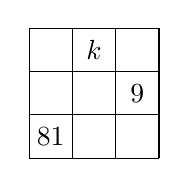
\begin{tikzpicture}[scale=0.55]
  \draw (0,0) grid (3,3);
  \node at (0.5, 0.5) {81};
  \node at (2.5, 1.5) {9};
  \node at (1.5, 2.5) {$k$};
\end{tikzpicture}
\end{minipage}
}

\Q{A、B 两地之间是山路，相距 150 千米，其中一部分是上坡路，其余是下坡路。某人骑电动车从 A 地到 B 地，再沿原路返回，去时用了 8 小时，返回时用了 7 小时。已知下坡路每小时行驶 30 千米，那么上坡路每小时行驶多少千米？}

\Q{
\begin{minipage}[c]{0.75\textwidth}
如图，$\triangle ABC$ 的面积是 72 平方厘米，$AD=DE=EC$，$F$ 是 $BC$ 中点，$FG=GC$，阴影部分的面积是\underline{\hspace{3em}}平方厘米。
\end{minipage}
\hfill
\begin{minipage}[c]{0.2\textwidth}
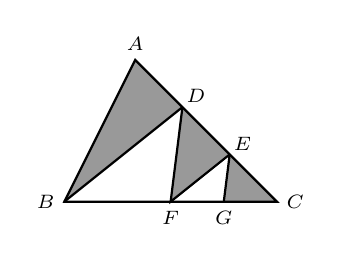
\begin{tikzpicture}[scale=0.45]
  \coordinate (B) at (0,0); \coordinate (C) at (6,0); \coordinate (A) at (2,4);
  \coordinate (D) at (3.333, 2.667); \coordinate (E) at (4.667, 1.333);
  \coordinate (F) at (3,0); \coordinate (G) at (4.5,0);
  \fill[gray!80] (A) -- (B) -- (D) -- cycle;
  \fill[gray!80] (D) -- (E) -- (F) -- cycle;
  \fill[gray!80] (E) -- (G) -- (C) -- cycle;
  \draw[thick] (A) -- (B) -- (C) -- cycle;
  \draw[thick] (B) -- (D); \draw[thick] (D) -- (F) -- (E); \draw[thick] (E) -- (G);
  \node[above] at (A) {\scriptsize $A$}; \node[left] at (B) {\scriptsize $B$}; \node[right] at (C) {\scriptsize $C$};
  \node[above right=-2pt] at (D) {\scriptsize $D$}; \node[above right=-2pt] at (E) {\scriptsize $E$};
  \node[below] at (F) {\scriptsize $F$}; \node[below] at (G) {\scriptsize $G$};
\end{tikzpicture}
\end{minipage}
}

\Q{桌上放有一张写有 61 的卡片，若从桌子的另一侧看去，却是 19。现在桌子上放着这样一道算术题：$86 + 18 + 89 + 6\Box + \Box8$。甲、乙两位同学面对面坐在桌子两侧，而他们计算这道数学题的结果恰好相同，则两个方格中应填的数字和是\underline{\hspace{3em}}。}

\Q{一列火车出发 1.5 小时后因故停车 0.5 小时，然后以原速的 $\dfrac{3}{4}$ 前进，最终到达目的地晚 2 小时。若出发 1.5 小时后又前进 90 公里再因故停车 0.5 小时，然后同样以原速的 $\dfrac{3}{4}$ 前进，则到达目的地仅晚 1.5 小时。那么整个路程为多少公里？}

\Qlast{老师在黑板上写了若干个从 1 开始的连续自然数：$1, 2, 3, 4, \dots$，后来擦掉其中的一个，剩下的数的平均数是 $13\dfrac{1}{3}$，擦掉的自然数是\underline{\hspace{3em}}。}

\end{OnePageEightFill}

% =========================================================
% 7.31
% =========================================================
\section*{7月31日作业（8道题当晚22:00前打卡）}
\begin{OnePageEightFill}

\Q{计算：$\displaystyle \frac{20 + \dfrac{1}{19}}{19 + \dfrac{1}{20}} - \frac{18 + \dfrac{1}{19}}{19 + \dfrac{1}{18}}$}

\Q{解方程组：$\begin{cases} 2x + y = 7 \\ \dfrac{x-4}{2} = \dfrac{y-6}{3} \end{cases}$}

\Q{
\begin{minipage}[c]{0.75\textwidth}
如图，为一个 3 行 3 列的表格，当空格内填上适当的数后，每行、每列以及每条对角线上的数字之和都是相等的，则 $k =$ \underline{\hspace{3em}}。
\end{minipage}
\hfill
\begin{minipage}[c]{0.2\textwidth}
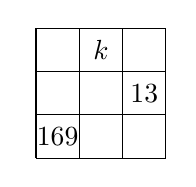
\begin{tikzpicture}[scale=0.55]
  \draw (0,0) grid (3,3);
  \node at (0.5, 0.5) {169};
  \node at (2.5, 1.5) {13};
  \node at (1.5, 2.5) {$k$};
\end{tikzpicture}
\end{minipage}
}

\Q{A、B 两地之间是山路，相距 360 千米，其中一部分是上坡路，其余是下坡路。某人骑电动车从 A 地到 B 地，再沿原路返回，去时用了 14 小时，返回时用了 12 小时。已知下坡路每小时行驶 45 千米，那么上坡路每小时行驶多少千米？}

\Q{
\begin{minipage}[c]{0.75\textwidth}
如图，$\triangle ABC$ 的面积是 84 平方厘米，$AD=DE=EC$，$F$ 是 $BC$ 中点，$FG=GC$，阴影部分的面积是\underline{\hspace{3em}}平方厘米。
\end{minipage}
\hfill
\begin{minipage}[c]{0.2\textwidth}
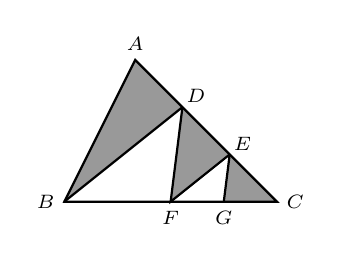
\begin{tikzpicture}[scale=0.45]
  \coordinate (B) at (0,0); \coordinate (C) at (6,0); \coordinate (A) at (2,4);
  \coordinate (D) at (3.333, 2.667); \coordinate (E) at (4.667, 1.333);
  \coordinate (F) at (3,0); \coordinate (G) at (4.5,0);
  \fill[gray!80] (A) -- (B) -- (D) -- cycle;
  \fill[gray!80] (D) -- (E) -- (F) -- cycle;
  \fill[gray!80] (E) -- (G) -- (C) -- cycle;
  \draw[thick] (A) -- (B) -- (C) -- cycle;
  \draw[thick] (B) -- (D); \draw[thick] (D) -- (F) -- (E); \draw[thick] (E) -- (G);
  \node[above] at (A) {\scriptsize $A$}; \node[left] at (B) {\scriptsize $B$}; \node[right] at (C) {\scriptsize $C$};
  \node[above right=-2pt] at (D) {\scriptsize $D$}; \node[above right=-2pt] at (E) {\scriptsize $E$};
  \node[below] at (F) {\scriptsize $F$}; \node[below] at (G) {\scriptsize $G$};
\end{tikzpicture}
\end{minipage}
}

\Q{桌上放有一张写有 61 的卡片，若从桌子的另一侧看去，却是 19。现在桌子上放着这样一道算术题：$89 + 61 + 88 + 6\Box + \Box8$。甲、乙两位同学面对面坐在桌子两侧，而他们计算这道数学题的结果恰好相同，则两个方格中应填的数字和是\underline{\hspace{3em}}。}

\Q{一列火车出发 2 小时后因故停车 1 小时，然后以原速的 $\dfrac{4}{5}$ 前进，最终到达目的地晚 2 小时。若出发 2 小时后又前进 160 公里再因故停车 1 小时，然后同样以原速的 $\dfrac{4}{5}$ 前进，则到达目的地仅晚 1.5 小时。那么整个路程为多少公里？}

\Qlast{老师在黑板上写了若干个从 1 开始的连续自然数：$1, 2, 3, 4, \dots$，后来擦掉其中的一个，剩下的数的平均数是 $15\dfrac{15}{29}$，擦掉的自然数是\underline{\hspace{3em}}。}

\end{OnePageEightFill}

\end{document}